Блок-схема разработанного программного комплекса имитационного
моделирования представлена на рисунке~\ref{fig:ui-block-schema}.

\begin{figure}[!h]
	\centering
	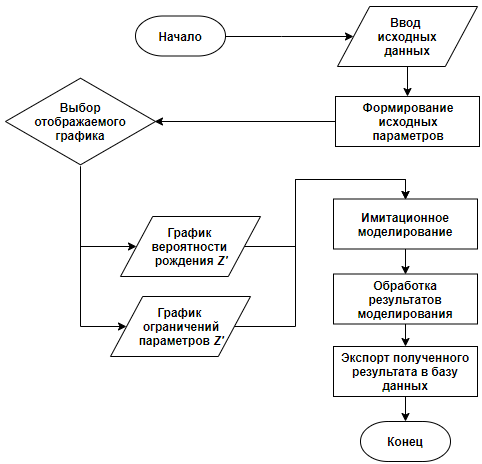
\includegraphics[width=\textwidth]{figures/ui-schema.png}
	\caption{Блок-схема программного комплекса имитационного моделирования}
	\label{fig:ui-block-schema}
\end{figure}

После открытия интерфейса приложения происходит начальная инициализация
(программный код представлен в приложении А), которая не видна
пользователю. Затем открывается главное окно интерфейса программного
комплекса.

Затем происходит формирование исходных параметров и пользователю
необходимо выбрать какой график необходимо вывести на экран. 

Если же
график не выбран, то будет выведена веб страница с описанием программного комплекса. После выбора Графика происходит имитационное моделирование по заданным параметрам. Далее
происходит обработка результатов моделирования и экспорт полученного
результата в базу данных, что позволяет не потерять накопленный результат и не затрачивать ресурсы на повторное моделирование. В качестве базы данных используется нереляционная база данных \textit{Redis}, отличающаяся от реляционных баз данных быстрым способом чтения и записи данных в виде ключ-значение. Так же используется сервис \textit{AWS ElastiCache}  разработанный компанией \textit{Amazon}, что позволяет огранизовать общий доступ для исследователей к результатам моделирования.